\section{Cartograms with Features}

{
\begin{figure}[b!]
    \centering
    \includegraphics[width=\columnwidth]{example-image-a}
    \caption{An overview of \software. Figure TBA.}
    \label{fig:overview}
\end{figure}
}

\algoref{alg:UpdateNodePosition} describes the overview of \software. We first load and render the CCG geospatial boundaries, for each CCG we compute the centroid where we render a node with $ \mathcal{S} $ as its size. We then apply the Fast Node Overlap Removal (VPSC) algorithm \cite{dwyer2006fast} recursively to remove overlaps. We chose VPSC over other node overlap removal algorithms since VPSC is able to provide spread minimization and node movement minimization while maintaining a good level of global shape preservation \cite{chen2020Node}. During each iteration, we test node trajectories (See \algoref{alg:check river crossing}) and move nodes that cross a river back to their previous position. A procedure ends when 1) no overlaps are present; 2) no nodes cross a river. We then increase $ \mathcal{S} $ by one pixel and repeat the algorithm until the entire map canvas is filled.

% \begin{noindent}

\begin{algorithm}[tb!]
    \caption{The procedure to update node positions by removing overlap and prevent nodes from crossing rivers.}\label{alg:UpdateNodePosition}
    \textbf{Global variables:} \\
    $ \mathbcal{L} \gets $ a list of nodes representing CCGs \\
    $ \mathcal{S} \gets $ the current size of all nodes \\
    $ \mathcal{S}_{max} \gets $ the maximum size of a node \\
    $ \mathcal{I} \gets $ the maximum number of iterations before a stalemate \\

    \textbf{Local variables:} \\
    $ \mathbcal{L}_{vpsc} \gets $ a list of nodes representing CCGs after running VPSC \\
    $ cross \gets $ the boolean for whether a node crossed a river \\

    \begin{algorithmic}[1]
        \Procedure{UpdateNodePosition}{}
        \While{$ \mathcal{S} < \mathcal{S}_{max} $}

        \State $ \mathbcal{L}_{vpsc} \gets $ RunVPSC ($ \mathbcal{L} $)

            \ForEach {$ \mathbcal{L}^i_{vpsc} \in \mathbcal{L}_{vpsc} $}

                \If {TranslateNode ($ \mathbcal{L}^i, \mathbcal{L}^i_{vpsc} $)}
                    \State $ cross \gets $ \Call{TestRiverCross}{$ \mathbcal{L}^i, \mathbcal{L}^i_{vpsc} $}

                    \If{$ cross = True $}
                        \State $ \mathcal{I} \gets \mathcal{I} + 1 $

                        \If{$ \mathcal{I} < \mathcal{I} $}
                            \State \Call{TranslateNode}{$ \mathbcal{L}^i $}
                        \Else
                            \State \Call{DeriveCorridor}{$ \mathbcal{L}^i, \mathbcal{L}^i_{vpsc} $}
                        \EndIf

                    \EndIf

                \EndIf

            \EndFor

        \EndWhile

        \State $ \mathcal{S} \gets \mathcal{S} ++$

        \EndProcedure
    \end{algorithmic}
\end{algorithm}


\begin{algorithm}[tb!]
    \caption{The procedure to update a single node's position.}\label{alg:move position}

    \textbf{Input:} \\
    $ \mathcal{N} \gets $ required, the node \\
    $ \mathcal{N}_{vpsc} \gets $ optional, the node after running VPSC \\

    \textbf{Output:} \\
    A boolean for whether the node's position is updated. \\

    \textbf{Local variables:} \\
    $ x,y \gets $ variables used to store coordinates \\

    \begin{algorithmic}[1]
        \Procedure{TranslateNode}{$ \mathcal{N}, \mathcal{N}_{vpsc} $}
        \If{$ \mathcal{N}.x = \mathcal{N}_{vpsc}.x $ and $ \mathcal{N}.y = \mathcal{N}_{vpsc}.y $}
            \item[] \Comment{Node position remains unchanged}
            \State \Return{$ False $}
        \EndIf

        \If{$ \mathcal{N}_{vpsc}$ is undefined } 
        \item[] \Comment{When optional parameter $ \mathcal{N}_{vpsc} $ is undefined}
        \item[] \Comment{Move the node back to its previous position}
            \State $ x \gets \mathcal{N}.previous.x,~y \gets \mathcal{N}.previous.y $
        \Else
            \State $ x \gets \mathcal{N}_{vpsc}.x,~y \gets \mathcal{N}_{vpsc}.y $
            \State $ \mathcal{N}.history.push(x, y) $
        \EndIf

        \State $ \mathcal{N}.x \gets x $
        \State $ \mathcal{N}.y \gets y $
        \State \Return{$ True $}
        \EndProcedure
    \end{algorithmic}
\end{algorithm}

%\end{noindent}

\subsection{River Cross Testing}

We use rivers as topological boundaries and prevent nodes from crossing them. When a node's position changes, we test if the node's trajectory intersects any segment of a river. See \algoref{alg:check river crossing}. A bounding box intersection test can be performed to reduce the number of line intersection detections required.

% \begin{noindent}
\begin{algorithm}[tb!]
    \caption{The procedure to test if a node crosses a river.}\label{alg:check river crossing}
    \textbf{Input:} \\
    $ \mathcal{N} \gets $ required, the node \\
    $ \mathcal{N}_{vpsc} \gets $ required, the node after running VPSC \\

    \textbf{Output:} \\
    A boolean for whether the node crosses a river. \\

    \textbf{Global variables:} \\
    $ \mathbcal{R} \gets $ a list of river edges \\

    \textbf{Local variables:} \\
    $ b_\mathcal{N}, b_{\mathcal{R}^i} \gets $ the bounding boxes for $\mathcal{N}$ and $\mathcal{R}^i$ \\
    $ b_{intersect} \gets $ a boolean for whether $b_\mathcal{N}$ intersects $b_\mathcal{R}^i$ \\
    $ e_\mathcal{N}, b_{\mathcal{R}^i} \gets $ the edges for $\mathcal{N}$ and $\mathcal{R}^i$ \\
    $ e_{intersect} \gets $ a boolean for whether $e_\mathcal{N}$ intersects $e_\mathcal{R}^i$ \\

    \begin{algorithmic}[1]
        \Procedure{TestRiverCross}{$ \mathcal{N}, \mathcal{N}_{vpsc} $}
        
        \ForEach{$ \mathcal{R}^i \in \mathbcal{R} $}
            \State $ b_{\mathcal{N}} \gets $ GenerateBoundingBox ($ \mathcal{N}, \mathcal{N}_{vpsc} $)
            \State $ b_{\mathcal{R}^i} \gets $ GenerateBoundingBox ($ \mathcal{R}^i $)
            \State $ b_{intersect} \gets $ TestBoundingIntersection ($ b_{\mathcal{N}}, b_{\mathcal{R}^i} $)
            
            \If{$ b_{intersect} = True $}
                \State $ e_{\mathcal{N}} \gets $ GenerateEdge ($ \mathcal{N}, \mathcal{N}_{vpsc} $)
                \State $ e_{\mathcal{R}^i} \gets $ GenerateEdge ($ \mathcal{R}^i $)
                \State $ e_{intersect} \gets $ TestEdgeIntersection ($ e_\mathcal{N}, e_{\mathcal{R}^i} $)
                
                \If{$ e_{intersect} = True $}
                    \State \Return{$ True $}
                \EndIf
            
                \EndIf
        \EndFor
        
        \State \Return{$ False $}
        \EndProcedure
    \end{algorithmic}
\end{algorithm}
%\end{noindent}

\subsection{Corridor Derivation}

As the VPSC always tries to produce an optimal node layout where node spread and movement are minimized, a node might be repeatedly translated between two positions due to the lack of available space, creating a stalemate situation, as shown in \figref{fig:stalemate}. In order to create space for VPSC to generate a new layout, we introduce a user-adjustable parameter, $ \mathcal{I} $, to test for stalemate. If a node is translated between two positions for more than $ \mathcal{I} $ iterations, it is considered to be in a stalemate. A stalemate triggers a corridor derivation which moves all nodes within the corridor by $ \mathcal{D} $ set by the user (See \figref{fig:corridor} and \algoref{alg:derive corridor}).

{
\begin{figure}[tb!]
    \centering
    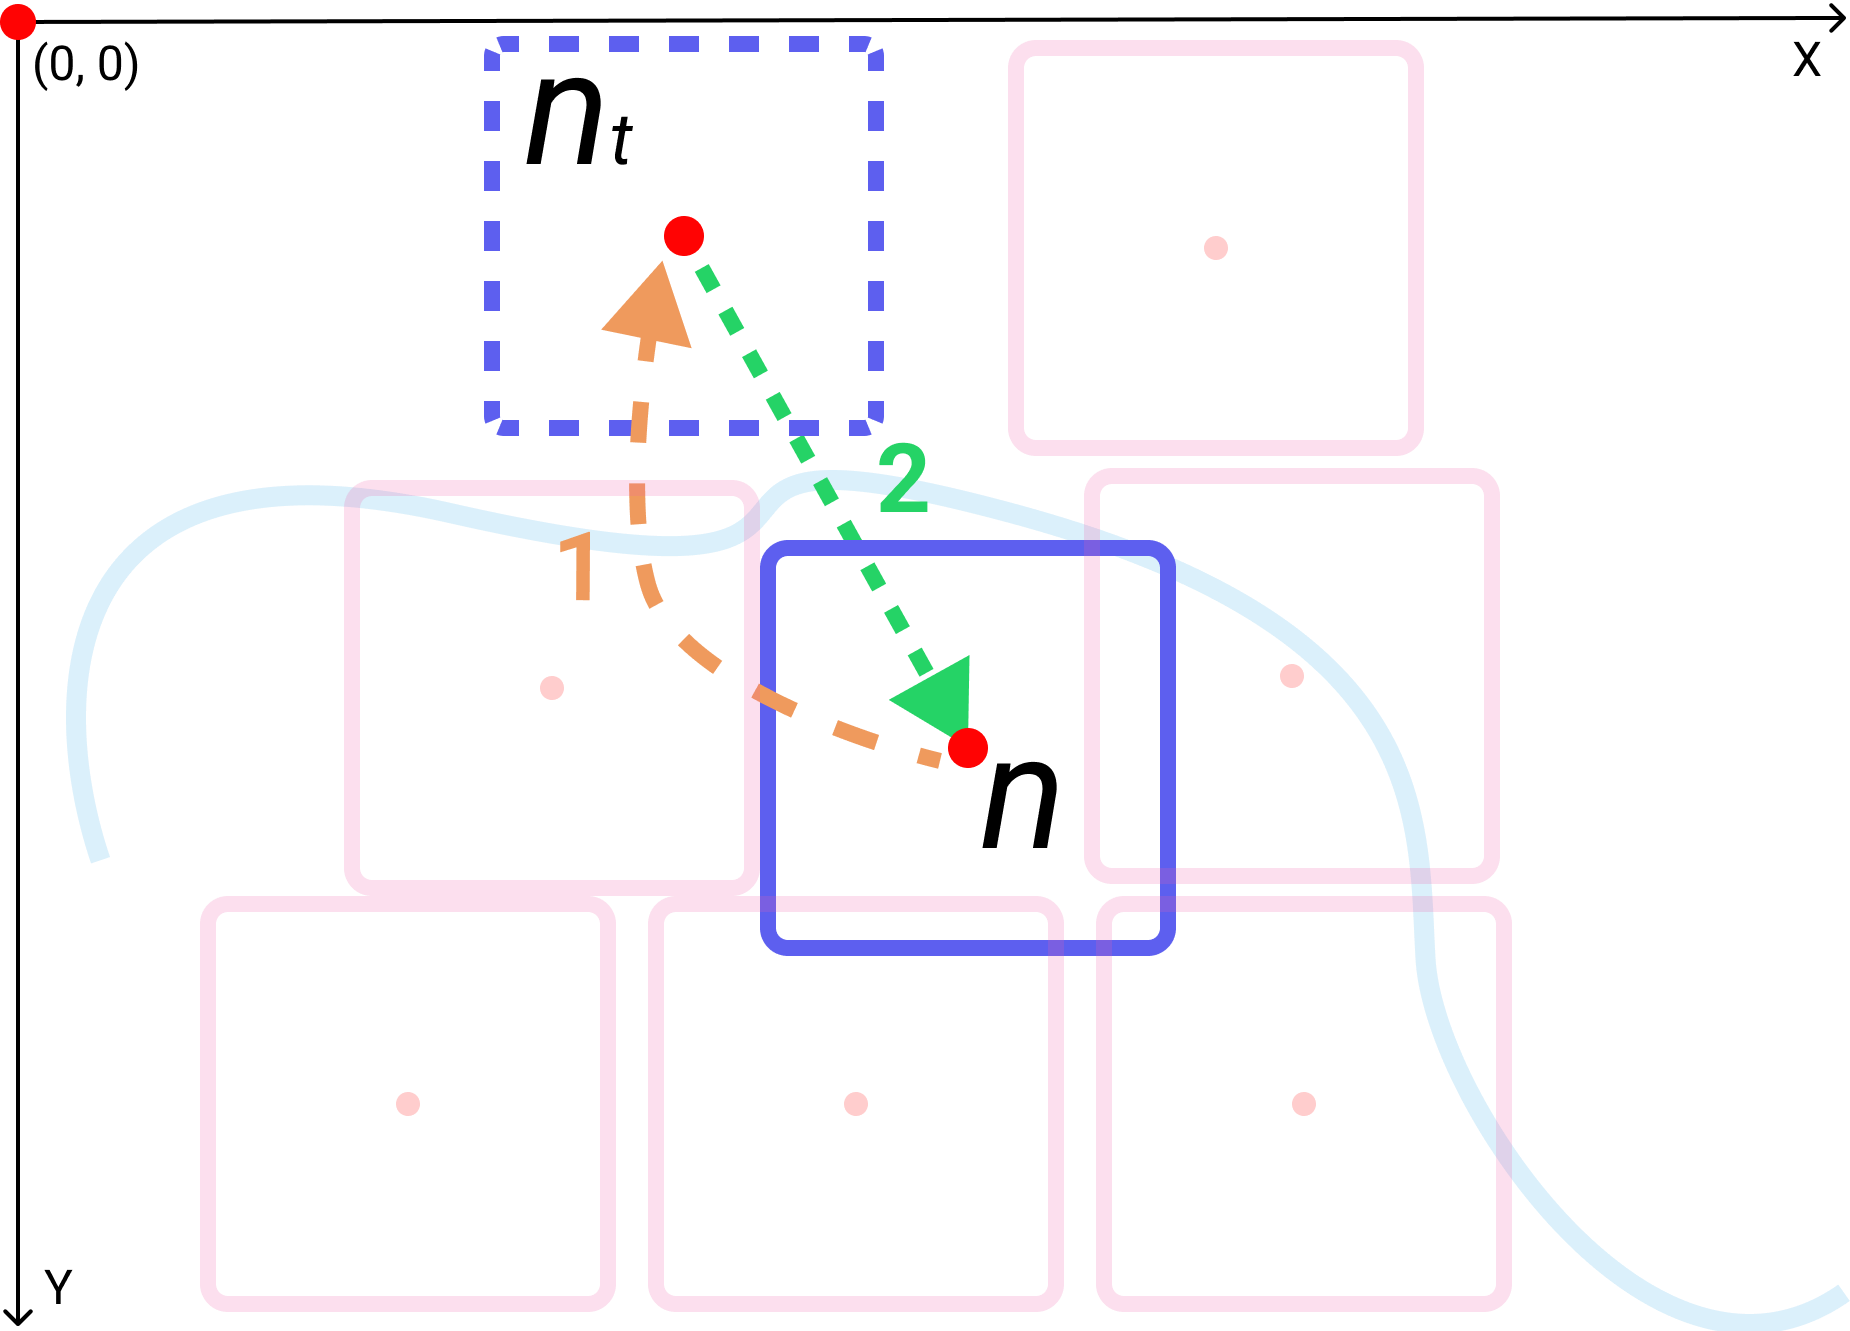
\includegraphics[width=\columnwidth]{figure/stalemate.png}
    \caption{A stalemate situation is when a node repeatedly translates between two positions (A and B) for more than $\mathcal{I}$ iterations. }
    \label{fig:stalemate}
\end{figure}
}

{
\begin{figure}[tb!]
    \centering
    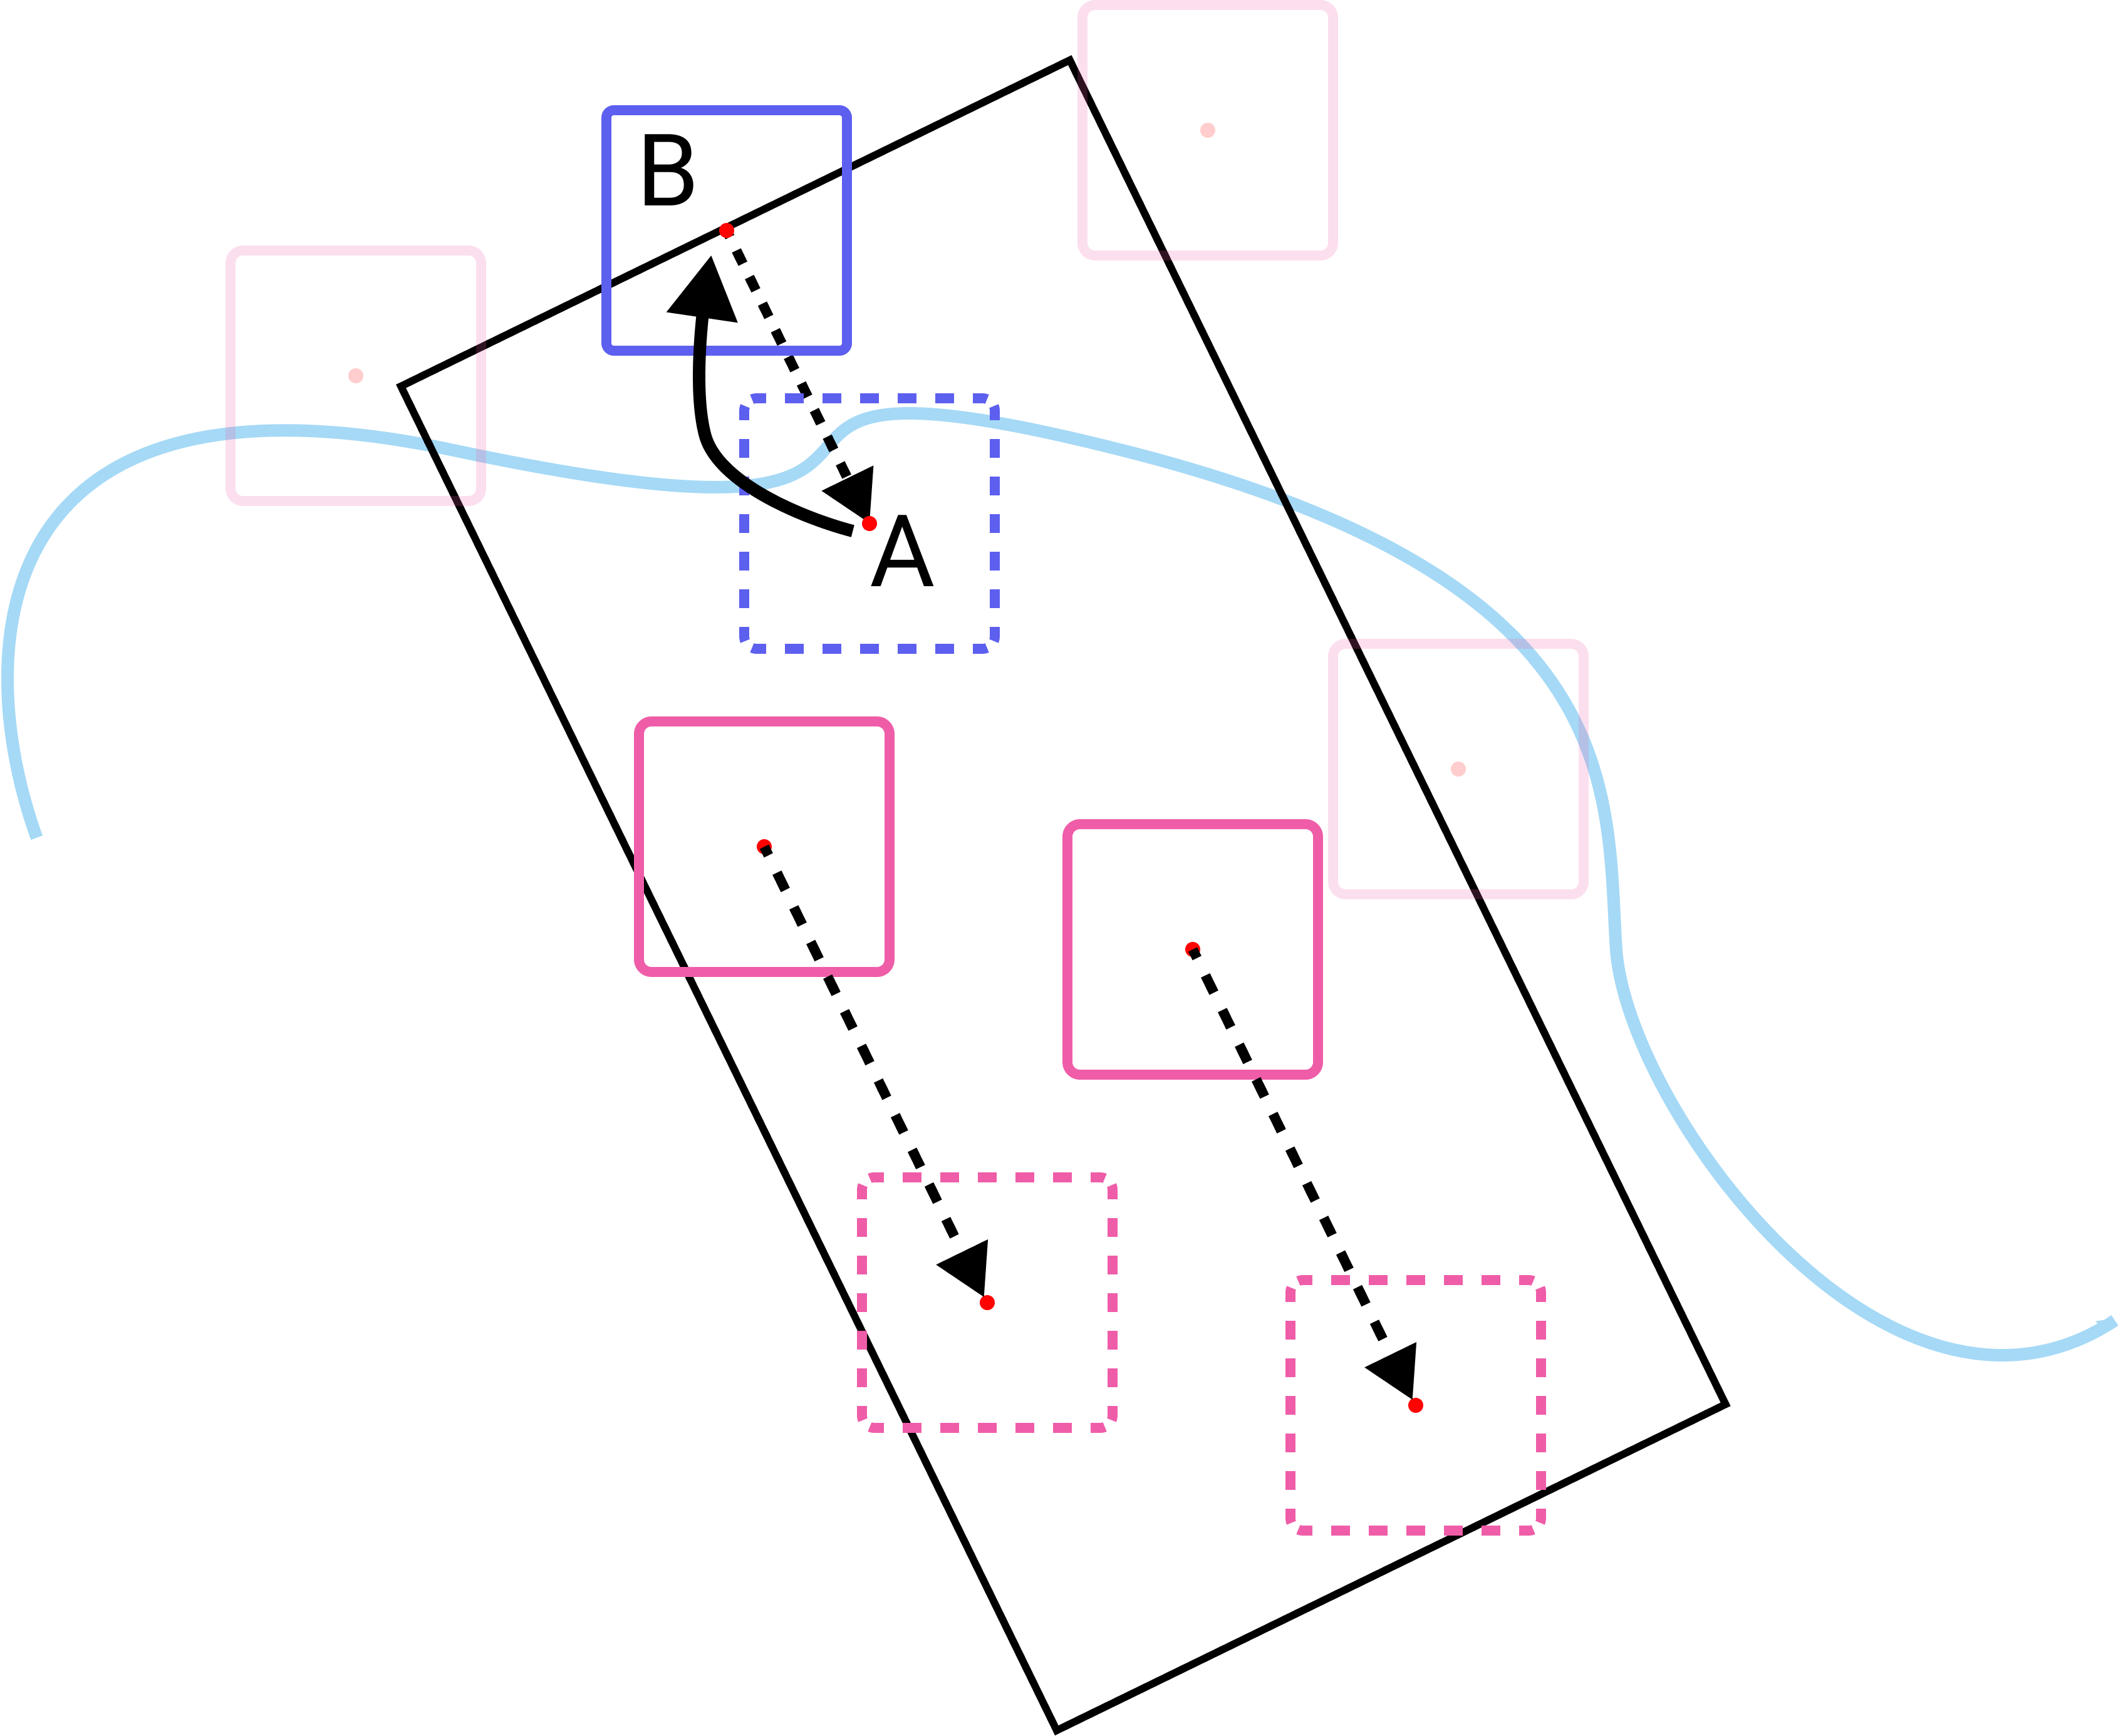
\includegraphics[width=\columnwidth]{figure/corridor.png}
    \caption{When a stalemate occurs, a corridor (black rectangular) is derived based on the current (A) and previous (B) positions of the node that crossed a river, as described in \algoref{alg:derive corridor}. All nodes within the corridor are moved by $ \mathcal{D} $ in the direction of $ \protect\overrightarrow{BA\strut} $. }
    \label{fig:corridor}
\end{figure}
}

% \begin{noindent}

\begin{algorithm}[tb!]
    \caption{The procedure to derive a corridor to move included nodes. We use a SVG canvas, where the point of origin (0,0) is located at the top left corner, with the x-axis extending to the right and the y-axis extending to the bottom, there is no negative axes.}\label{alg:derive corridor}

    \textbf{Input:} \\
    $ \mathcal{N} \gets $ required, the node current state \\
    $ \mathcal{N}_{p} \gets $ required, the node's previous state \\

    \textbf{Output:} \\
    A boolean for whether the node's position is updated. \\

    \textbf{Global variables:} \\
    $ \mathcal{C}_l \gets $ the length of a corridor \\
    $ \mathcal{C}_w \gets $ the width of a corridor \\
    $ \mathcal{D} \gets $ the distance to move nodes within the corridor \\

    \textbf{Local variables:} \\
    $ slope \gets $ the slope of $ \overrightarrow{\mathcal{N}\mathcal{N}_{p}\strut} $ \\
    $ e_{p} \gets $ an edge perpendicular at $ \mathcal{N} $ on $ \overrightarrow{\mathcal{N}\mathcal{N}_{p}\strut} $ \\
    $ e_{s^1} \gets $ a perpendicular edge at the start of $ e_{p} $ \\
    $ e_{s^2} \gets $ a perpendicular edge at the end of $ e_{p} $ \\
    $ corridor \gets $ a rectangular formed by $ e_p $, $ e_{s^1} $ and $ e_{s^2} $ \\
    $ n_{in} \gets $ a node located inside $ corridor $ \\
    $ e_{d} \gets $ an edge connecting $ \mathcal{N} $ and its destination \\

    \begin{algorithmic}[1]
        \Procedure{DeriveCorridor}{$ \mathcal{N}, \mathcal{N}_{p} $}
            \State TranslateNode ($ \mathcal{N} $)

            \State $ \Delta x \gets \mathcal{N}.x - \mathcal{N}_{p}.x,~ \Delta y \gets \mathcal{N}.y - \mathcal{N}_{p}.y $

            \State $ slope \gets \frac{\Delta x}{\Delta y}$

            \State $ e_{p} = $ \Call{DeriveEdge}{$ \frac{-1}{ slope } $, $ \mathcal{N} $, $ \mathcal{C}_w $}
            \State $ e_{s^1} = $ \Call{DeriveEdge}{$ slope $, $ e_{p}.a $, $ \mathcal{C}_l $, $ True $}
            \State $ e_{s^2} = $ \Call{DeriveEdge}{$ slope $, $ e_{p}.b $, $ \mathcal{C}_l $, $ True $}
            \State $ corridor \gets
                \begin{bmatrix}
                    e_{p}.a &
                    e_{p}.b \\

                    e_{s^1}.a &
                    e_{s^2}.b \\
                \end{bmatrix} $

            \ForEach{$ {n}_{in}^i $ inside $ corridor $}
                \State $ {n}_{in}^i.dx \gets \Delta x $, $ {n}_{in}^i.dy \gets \Delta y $
                \State $ e_{d} = $ \Call{DeriveEdge}{$ slope $, $ {n}_{in}^i $, $ \mathcal{D} $}

                \State TranslateNode ($ {n}_{in}^i, e_{d}.b $)
            \EndFor
        \EndProcedure
    \end{algorithmic}
\end{algorithm}

%\end{noindent}

% \begin{noindent}

\begin{algorithm}[tb!]
    \caption{The procedure to derive an edge based on a slope and a point.}\label{alg:derive corridor point}
    \textbf{Input:} \\
    $ Slope \gets $ the slope used to derive an edge \\
    $ Point \gets $ the point used to derive an edge \\
    $ Length \gets $ the length of the derived edge \\
    $ IsSideEdge \gets $ the boolean used to determine the edge's type \\

    \textbf{Output:} \\
    An edge that passes through a given point with the given slope. \\

    \textbf{Local variables:} \\
    $ a,b \gets $ variables used to store coordinates \\
    $ \Delta x, \Delta y \gets $ the differences in $ x, y $ \\

    \begin{algorithmic}[1]
        \Procedure{DeriveEdge}{$ Slope, Point, Length, IsSideEdge $}

        \Switch{$Slope$}
            \Case{$0$}
                \If{$ IsSideEdge = True $}
                    \State $ a.x \gets Point.x $
                \Else
                    \State $ a.x \gets Point.x + Length $
                \EndIf
                \State $ a.y \gets Point.y $

                \If{$ Point.dx < 0 $}
                    \State $ a.x \gets Point.x + Length $
                \Else
                    \State $ a.x \gets Point.x - Length $
                \EndIf
                \State $ b.x \gets Point.x - Length $,~$ b.y \gets Point.y $
            \EndCase
            \Case{$ \infty $ or $ -\infty $}
                \State $ a.x \gets Point.x $

                \If{$ IsSideEdge = True $}
                    \State $ a.y \gets Point.y $
                \Else
                    \State $ a.y \gets Point.y + Length $
                \EndIf

                \If{$ Point.dy < 0 $}
                    \State $ a.y \gets Point.y + Length $
                \Else
                    \State $ a.y \gets Point.y - Length $
                \EndIf

                \State $ b.x \gets Point.x $,~$ b.y \gets Point.y - Length $
            \EndCase
            \Default
                \State $ \Delta x = \sqrt{\frac{Length}{{1+Slope^2}}}$,~ $ \Delta y = Slope \cdot \Delta x $
                \If{$ IsSideEdge = True $}
                    \State $ a.x \gets Point.x $,~$ a.y \gets Point.y $
                \Else
                    \State $ a.x \gets Point.x + \Delta x $,~$ a.y \gets Point.y + \Delta y $
                \EndIf

                \If{$ Point.dx > 0 $ and $ Slope = 1 $ and $ IsSideEdge = True $}
                    \State $ b.x \gets Point.x + \Delta x $,~$ b.y \gets Point.y + \Delta y $
                \Else
                    \State $ b.x \gets Point.x - \Delta x $,~$ b.y \gets Point.y - \Delta y $
                \EndIf
                
            \EndDefault

        \EndSwitch

        \State \Return{$ a, b $}

        \EndProcedure

    \end{algorithmic}
\end{algorithm}

%\end{noindent}